\documentclass{article}
\usepackage{polski}
\usepackage[utf8]{inputenc}
\usepackage{mathtools}
\usepackage{graphicx}

\graphicspath{{img/}}

\begin{document}


\section{Dataset generation}
To generate dataset I used the same method as in the previous assignment. This time I combined 9 circular dataset, with centers in a 3 x 3 grid. I looked like this:

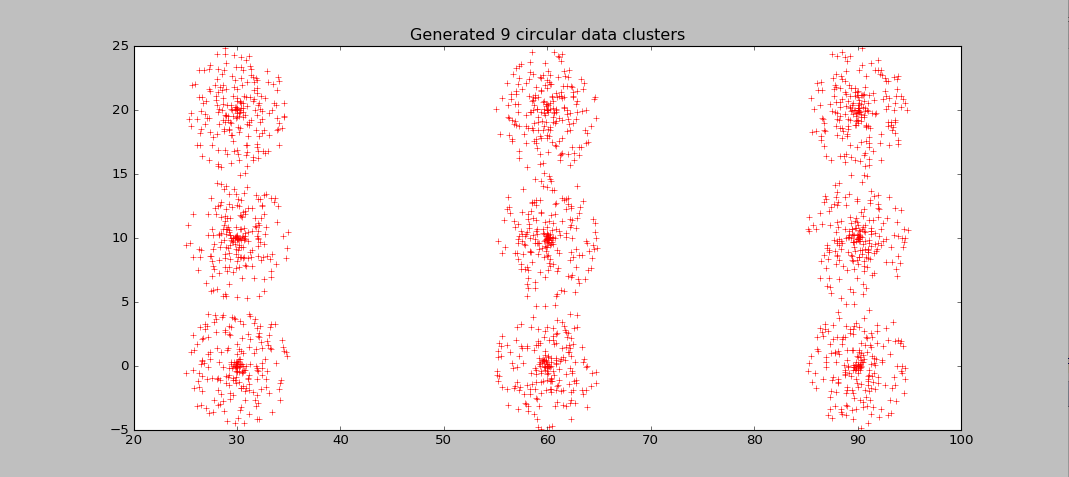
\includegraphics[width=\textwidth]{datasets}


\section{Initilization methods}
Then I ran k-means algorithm with four different initialization methods :

\begin{itemize}
  \item Fully random
  \item Forgy
  \item Random partition
  \item k-means++
\end{itemize}

\section{Results}

To measure the quality of the algorithm (with different initialization methods) I decided to use silhouette score
as a metric. I chose it because it is already conveniently imlemented in sklearn.metrics module.
Generally the higher silhouette score the better performed the clustering method.

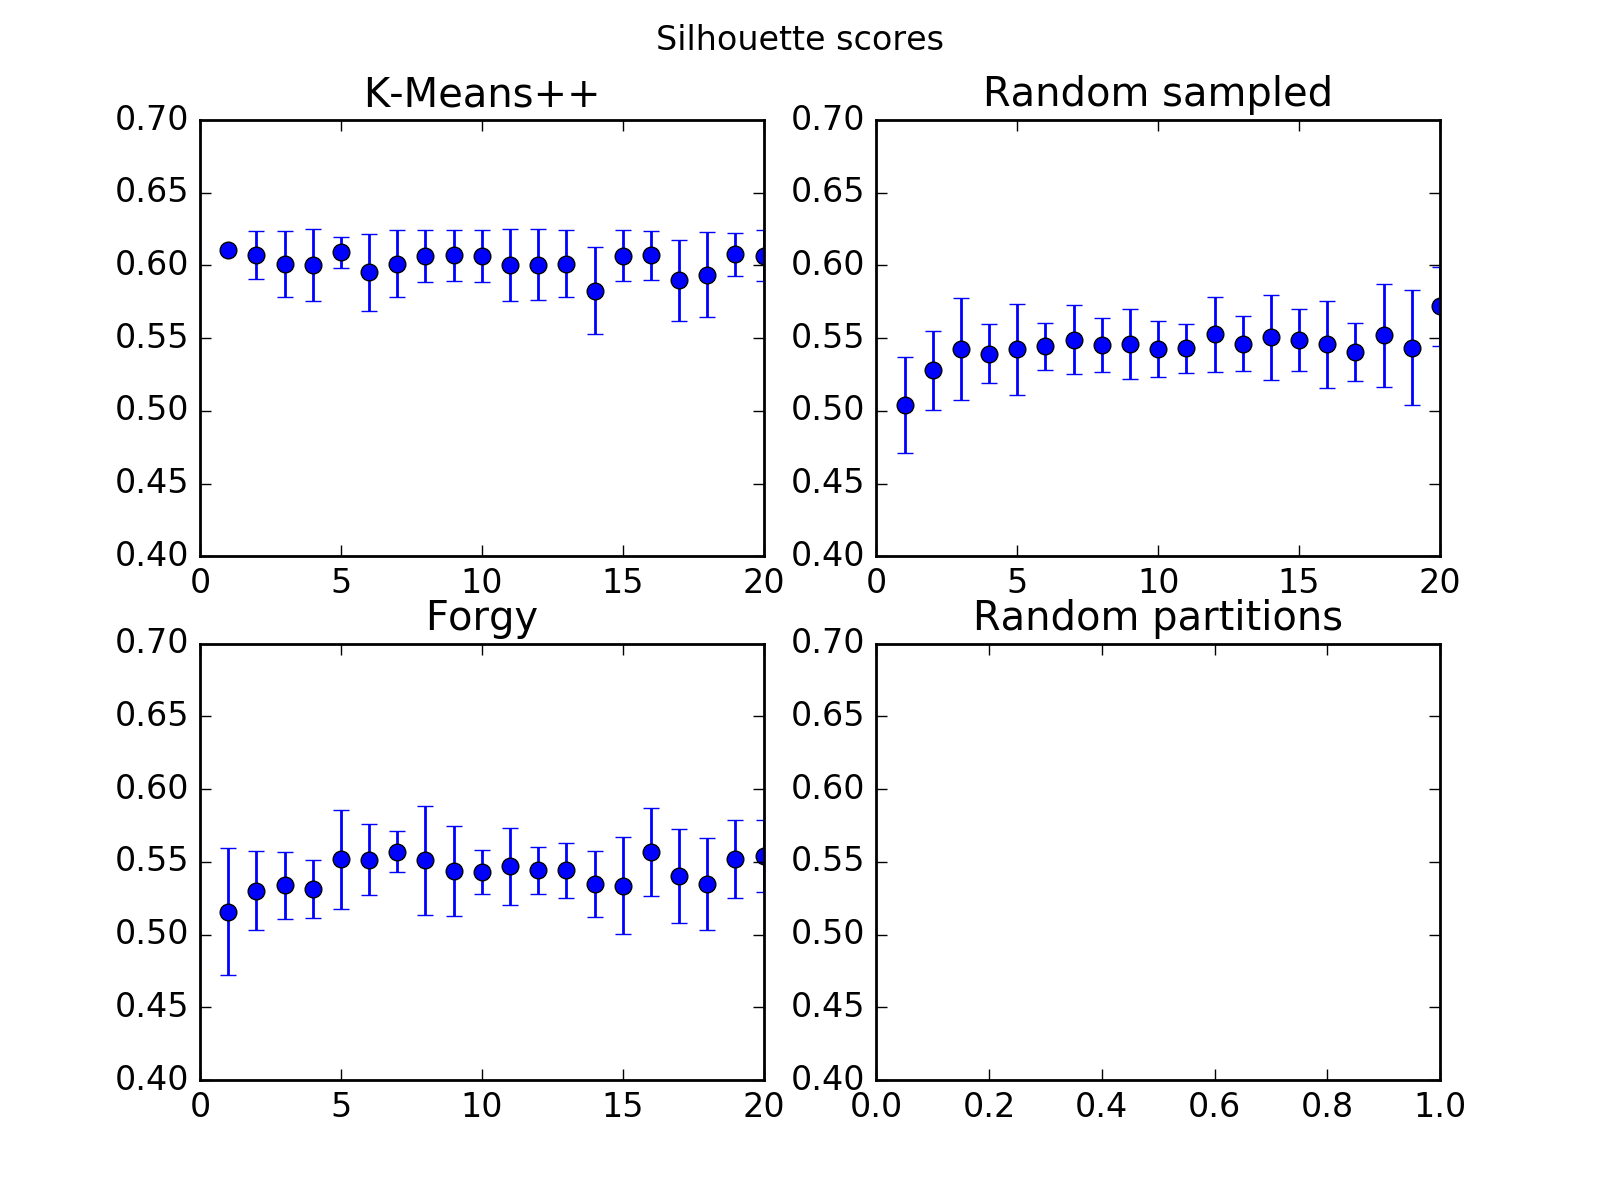
\includegraphics[width=\textwidth]{clustering}

\section{Discussion}

The results show clearly that the k-means++ has the best score. It seams that both forgy and random
initializations yield perform nearly the same, but random init has greater variance between runs. It was expected since Forgy uses only points existing in dataset as initial cluster centers, while in random
the whole space is available.

\end{document}
